\documentclass[14pt]{beamer}

% use the metropolis theme, with a black main color
\usetheme[titleformat = smallcaps]{metropolis}
\setbeamercolor{normal text}{fg=black, bg=white}

% add fade transition
\addtobeamertemplate{background canvas}{\transfade[duration=0.5]}{}

% set a frame footer to fit the purpose of the presentation
\setbeamertemplate{frame footer}{SOČ 2019}

% change frame footer and numbering color to gray to make it less intrusive
\setbeamercolor{frame footer}{fg=gray}
\setbeamercolor{frame numbering}{fg=gray}

% change \today formatting to d. m. yyyy
\usepackage[dmyyyy]{datetime}
\renewcommand{\dateseparator}{. }


% GRAPHICS %
%-========-%
\usepackage{graphicx}     % graphics package
\graphicspath{ {./images/} } % path to images

\usepackage{float} % floats in correct position (the [H] option)

\usepackage{subcaption} % for subfigures

\setlength{\fboxsep}{0pt}    % image border separation
\setlength{\fboxrule}{0.5pt} % image border thickness


% GRAPHS, CHARTS %
%-==============-%
\usepackage{pgf-pie} % pie charts

% change pie chart number separator from dot to comma
\usepackage{siunitx}
\sisetup{
  output-decimal-marker={,},
  group-separator={\,},
}
\def\ScanPercentage#1\afternumber{\SI{#1}{\percent}}

\usepackage{pgfplots} % bar charts


% CAPTIONS %
%-========-%
\usepackage[font=footnotesize,       % 10pt captions
            justification=centering, % center the captions
            figurename=Obr.,         % picture captions are "Obr."
            tablename=Tab.]{caption} % table captions are "Tab."


% TABLES          %
% requires: float %
%-===============-%
\usepackage{booktabs} % table formatting
\usepackage{multirow} % for creating multirow tables


% MATH %
%-====-%
\usepackage{amsmath, amstext} % for typesetting math
\DeclareMathSymbol{.}{\mathord}{letters}{"3B} % change dot in math to a comma

% FONT AND ENCODING %
%-=================-%
\usepackage{fontawesome5} % use FontAwesome 5 for icons
\newfontfamily\mathfont{CMU Serif} % will be used for \LaTeX and \KaTeX commands
\usefonttheme[onlymath]{serif} % use a serif font for math


% LISTS %
%-=====-%
% remember the old list margins for later use
\newlength{\originalmarginlength}
\setlength{\originalmarginlength}{\leftmargini}

% set left list margins to 0
\setlength\leftmarginiii{\leftmarginii}
\setlength\leftmarginii{\leftmargini}
\setlength\leftmargini{0em}


% define KaTeX logo
\makeatletter
\DeclareRobustCommand{\KaTeX}{%
  K\kern -.19em
  {\sbox \z@ T\vbox to\ht \z@ {\hbox{%
  \check@mathfonts
  \fontsize\sf@size\z@
  \selectfont A}%
  \vss}%
}\kern -.15em
\TeX}
\makeatother

% ---------------------------------------------------------------------------- %

% title page settings
\title{\makebox[\linewidth]{Robotika jednoduše}}
\setbeamerfont{title}{size=\huge} % center the title

\date{\today}
\author{Tomáš Sláma}
\institute{Gymnázium Turnov}

\begin{document}
  \maketitle

  \begin{frame}{Motivace}
    \begin{itemize}
      \item<+-> praktické uplanění robotiky v dnešním světě
      \item<+-> nedostatek přístupných materiálů
      \item<+-> centralizovaný zdroj informací
    \end{itemize}
  \end{frame}

  \section{Technické provedení}

  \begin{frame}{Generování stránky}
    \begin{itemize}
      \item<+-> \textbf{Jekyll} -- generátor statických webových stránek
      \item<+-> zdrojový kód ze souborů prostého textu
    \end{itemize}

    \begin{columns}[T, onlytextwidth]
      \footnotesize
      \column<+->{0.5\textwidth}
        \begin{center}
          \faIcon{plus}
        \end{center}
        \begin{itemize}[<+- | alert@+>]
          \item vyšší bezpečnost
          \item jednoduchost verzování
        \end{itemize}
      \column<+->{0.5\textwidth}
        \begin{center}
          \faIcon{minus}
        \end{center}
        \begin{itemize}[<+- | alert@+>]
          \item žádný dynamický obsah
          \item obtížnost nastavení
        \end{itemize}
    \end{columns}
  \end{frame}

  \begin{frame}{Multiplatformnost}
    \begin{minipage}[b]{\textwidth}
      \begin{table}[H]
        \caption{Funkčnost stránky na různých platformách}
        \scriptsize
        \centering
        \begin{tabular}{@{}rccccccccccccc@{}} \toprule
          & \multicolumn{6}{c}{Stolní počítač} & \phantom{abc} & \multicolumn{6}{c}{Mobilní zařízení} \\
            \cmidrule{2-7} \cmidrule{9-14}
           & \faIcon{firefox} & \faIcon{chrome} & \faIcon{internet-explorer} & \faIcon{edge} & \faIcon{safari} & \faIcon{opera}
          && \faIcon{firefox} & \faIcon{chrome} & \faIcon{internet-explorer} & \faIcon{edge} & \faIcon{safari} & \faIcon{opera}\\
            \midrule
          Obrázky     & \faIcon{check} & \faIcon{check} & \faIcon{check} & \faIcon{check} & \faIcon{check} & \faIcon{check}
          && \faIcon{check} & \faIcon{check} & \faIcon{minus} & \faIcon{check} & \faIcon{check} & \faIcon{check} \\
          Rovnice     & \faIcon{check} & \faIcon{check} & \faIcon{check} & \faIcon{check} & \faIcon{check} & \faIcon{check}
          && \faIcon{check} & \faIcon{check} & \faIcon{minus} & \faIcon{check} & \faIcon{check} & \faIcon{check} \\
          Vizualizace & \faIcon{check} & \faIcon{check} & \faIcon{times} & \faIcon{check} & \faIcon{check} & \faIcon{check}
          && \faIcon{check} & \faIcon{check} & \faIcon{minus} & \faIcon{check} & \faIcon{check} & \faIcon{check} \\
          Formátování & \faIcon{check} & \faIcon{check} & \faIcon{check} & \faIcon{check} & \faIcon{check} & \faIcon{check}
          && \faIcon{check} & \faIcon{check} & \faIcon{minus} & \faIcon{check} & \faIcon{check} & \faIcon{check} \\
            \bottomrule
        \end{tabular}
      \end{table}
    \end{minipage}
  \end{frame}

  \begin{frame}{Automatizace provozu}
    \begin{itemize}
      \item<+-> \textbf{Python} -- skriptovací jazyk
      \item<+-> rozsáhlá standardní knihovna
      \item<+-> vysoká míra abstrakce
    \end{itemize}

    % temporarily set the margin to its original value to indent the enumerate
    \setlength\leftmargini{\originalmarginlength}

    \begin{enumerate}[<+- | alert@+>]
      \item upload stránky přes FTP
      \item generování souboru sitemap.xml
      \item převod do PDF
      \item komprimace obrázků
      \item minimalizace zdrojového kódu
    \end{enumerate}

    \setlength\leftmargini{0em}
  \end{frame}


  \section{Návštěvnost}

  \begin{frame}{Pohlaví a věk}
    \begin{figure}
      \begin{minipage}[b]{0.475\textwidth}
        \scriptsize
        \centering
        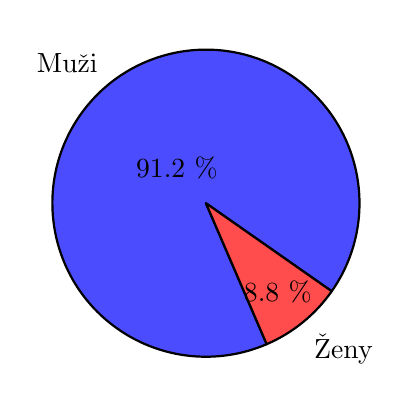
\begin{tikzpicture}[scale=0.65]
          \pie[color={blue!70, red!70}, rotate=-35, before number=\ScanPercentage, after  number ={ }\%,]{91.2/Muži, 8.8/Ženy}
        \end{tikzpicture}
        \captionof{figure}{Pohlaví návštěvníků}
        \label{img:Pohlaví návštěvníků}
      \end{minipage}\hfill
      \begin{minipage}[b]{0.475\textwidth}
        \scriptsize
        \centering
        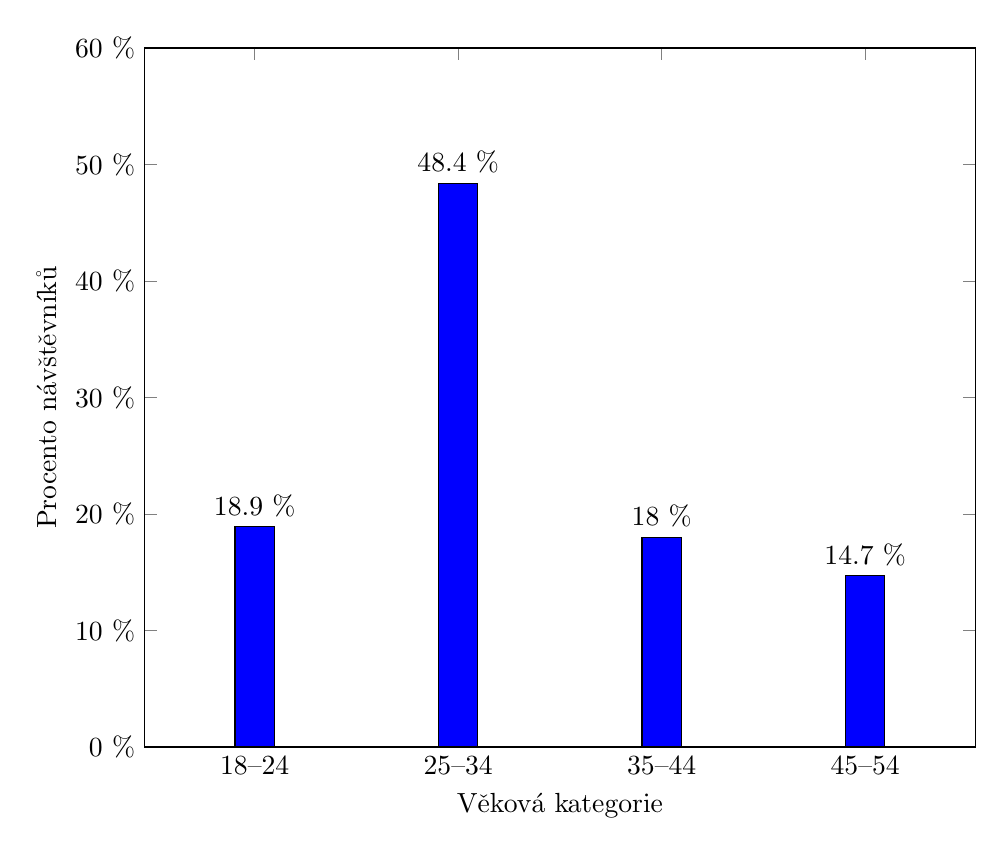
\begin{tikzpicture}
          \begin{axis}[
            symbolic x coords={18--24, 25--34, 35--44, 45--54},
            xtick=data,
            ylabel={Procento návštěvníků},
            xlabel={Věková kategorie},
            bar width=0.5cm,
            width=\textwidth,
            enlarge x limits=0.18,
            ymin=0, ymax=60,
            nodes near coords={\pgfmathprintnumber\pgfplotspointmeta{ }\%},
            yticklabel={\pgfmathparse{\tick}\pgfmathprintnumber{\pgfmathresult}{ }\%},]
            \addplot[ybar,fill=blue] coordinates {
              (18--24, 18.9)
              (25--34, 48.4)
              (35--44, 18.0)
              (45--54, 14.7)
            };
          \end{axis}
        \end{tikzpicture}
        \captionof{figure}{Věk návštěvníků}
        \label{img:Věk návštěvníků}
      \end{minipage}
    \end{figure}
  \end{frame}


  \begin{frame}{Prohlížeč a lokace}
    \begin{figure}
      \begin{minipage}[b]{0.5\textwidth}
        \begin{table}[H]
          \caption{Lokace návštěvníků}
          \scriptsize
          \centering
          \begin{tabular}{lr}
            \toprule
            \emph{Země} & \emph{Návštěvníci} \\
            \midrule
            Spojené státy      & \num{240} \\
            Česká republika	   & \num{35} \\
            Spojené království & \num{20} \\
            Kanada             & \num{17} \\
            Německo            & \num{10} \\
            Japonsko           & \num{10} \\
            Čína               & \num{8} \\
            Indie              & \num{8} \\
            Španělsko          & \num{7} \\
            Nizozemí           & \num{7} \\
            \bottomrule
          \end{tabular}
        \end{table}
      \end{minipage}\hfill
      \begin{minipage}[b]{0.5\textwidth}
        \begin{table}[H]
          \caption{Prohlížeč návštěvníků}
          \scriptsize
          \centering
          \begin{tabular}{lr}
            \toprule
            \emph{Prohlížeč} & \emph{Návštěvníci} \\
            \midrule
            Chrome            & \num{226} \\
            Firefox	          & \num{111} \\
            Safari            & \num{85} \\
            Android Webview   & \num{14} \\
            Internet Explorer & \num{6} \\
            Opera             & \num{6} \\
            Edge              & \num{5} \\
            Samsung Internet  & \num{5} \\
            Neurčeno          & \num{4} \\
            Cốc Cốc           & \num{1} \\
            \bottomrule
          \end{tabular}
        \end{table}
      \end{minipage}
    \end{figure}
  \end{frame}

  \appendix

  {\setbeamertemplate{frame footer}{}
  \begin{frame}[standout]
    Děkuji za pozornost
  \end{frame}}
\end{document}
